% paper/sections/12g_nonuniform_grid.tex
%
% §12.5b  界面適合格子の NS 結合検証
% ═══════════════════════════════════════════════════════════════════════════════
\subsection{界面適合格子の NS パイプライン結合検証}
\label{sec:nonuniform_grid_ns}
% ═══════════════════════════════════════════════════════════════════════════════

% ─────────────────────────────────────────────────────────────────────────────
\subsubsection{静止液滴 NS 結合テスト：格子収束性}
\label{sec:nonuniform_ns_static_droplet}
% ─────────────────────────────────────────────────────────────────────────────

\noindent\textbf{目的：}
§~\ref{sec:grid_ale} で設計した界面適合格子が NS パイプライン全体と結合した際に
静止液滴の質量保存・寄生流れ・Laplace 圧力に与える影響を定量化する．

\noindent\textbf{評価対象：}
格子密度関数 $\omega(\phi) = 1 + (\alpha{-}1)\,\varepsilon_g\,\delta_\varepsilon^*(\phi)$
（$\alpha = 2$，界面適合，$N_{g,\text{cells}} = 4$）と一様格子（$\alpha = 1$）を同一条件下で比較する．
格子密度幅には計算空間セル数定義（式~\eqref{eq:eps_g_xi}）を使用する．
§~\ref{sec:verify_ns_grid_rebuild} で短時間（100 ステップ，$N{=}32$）の安定性は既確認のため，
本節では解像度を $N = 32, 48, 64$ に拡張し，200 ステップの
静止液滴テストで格子収束性を評価する．

\noindent\textbf{手順とパラメタ：}
\begin{itemize}[noitemsep]
  \item $R = 0.25$，$\rho_l/\rho_g = 10$，$\sigma = 1.0$，$\mu = 0.05$，壁境界
  \item $\Delta t$ は CFL 安定条件（$\mathrm{CFL} = 0.10$）で自動設定
  \item 一様（$\alpha = 1$）と界面適合（$\alpha = 2$）を同一条件で比較
  \item 一様格子では既存設定を維持し 2 ステップ毎に再初期化，
        非一様格子では再初期化を無効化
\end{itemize}

\noindent
非一様格子での再初期化無効化は実装上の制約による：
現行の再初期化器は一様格子幅を仮定しており，非一様格子では
$3\times10^{-2}$--$2\times10^{-1}$ の質量ずれを生じる
（格子リビルド自体はそのずれを保存するのみ）．

\noindent\textbf{結果：}

\begin{table}[htbp]
\centering
\caption{静止液滴の格子収束性：一様格子 vs 界面適合格子（$N_{g,\text{cells}} = 4$，$t = 200\Delta t$）．
$N = 32$ は両格子とも CSF 解像度不足により発散したため除外\textsuperscript{$\dagger$}．}
\label{tab:nonuniform_ns_convergence}
\renewcommand{\arraystretch}{1.3}
\begin{tabular}{ccccccc}
\toprule
$N$ & $\alpha$ & 再初期化間隔 & $\max|\bu|$ & $\Delta p$ 相対誤差 & $|\Delta M|/M_0$ & $h_{\min}$ \\
\midrule
48 & 1 & 2 & $4.36 \times 10^{-1}$ & 5.9\%  & $1.86 \times 10^{-4}$ & 0.0208 \\
48 & 2 & off & $5.59 \times 10^{-3}$ & \textbf{0.10\%} & $1.67 \times 10^{-5}$ & 0.0171 \\
\midrule
64 & 1 & 2 & \multicolumn{4}{c}{発散\textsuperscript{$\dagger$}} \\
64 & 2 & off & $8.83 \times 10^{-1}$ & 0.88\% & $4.85 \times 10^{-4}$ & 0.0126 \\
\midrule
\multicolumn{7}{l}{\footnotesize \textsuperscript{$\dagger$}$\max|\bu| > 10^{6}$，
CSF の界面近傍解像度が不足し 200 ステップ到達前に発散．} \\
\bottomrule
\end{tabular}
\end{table}

\begin{figure}[htbp]
\centering
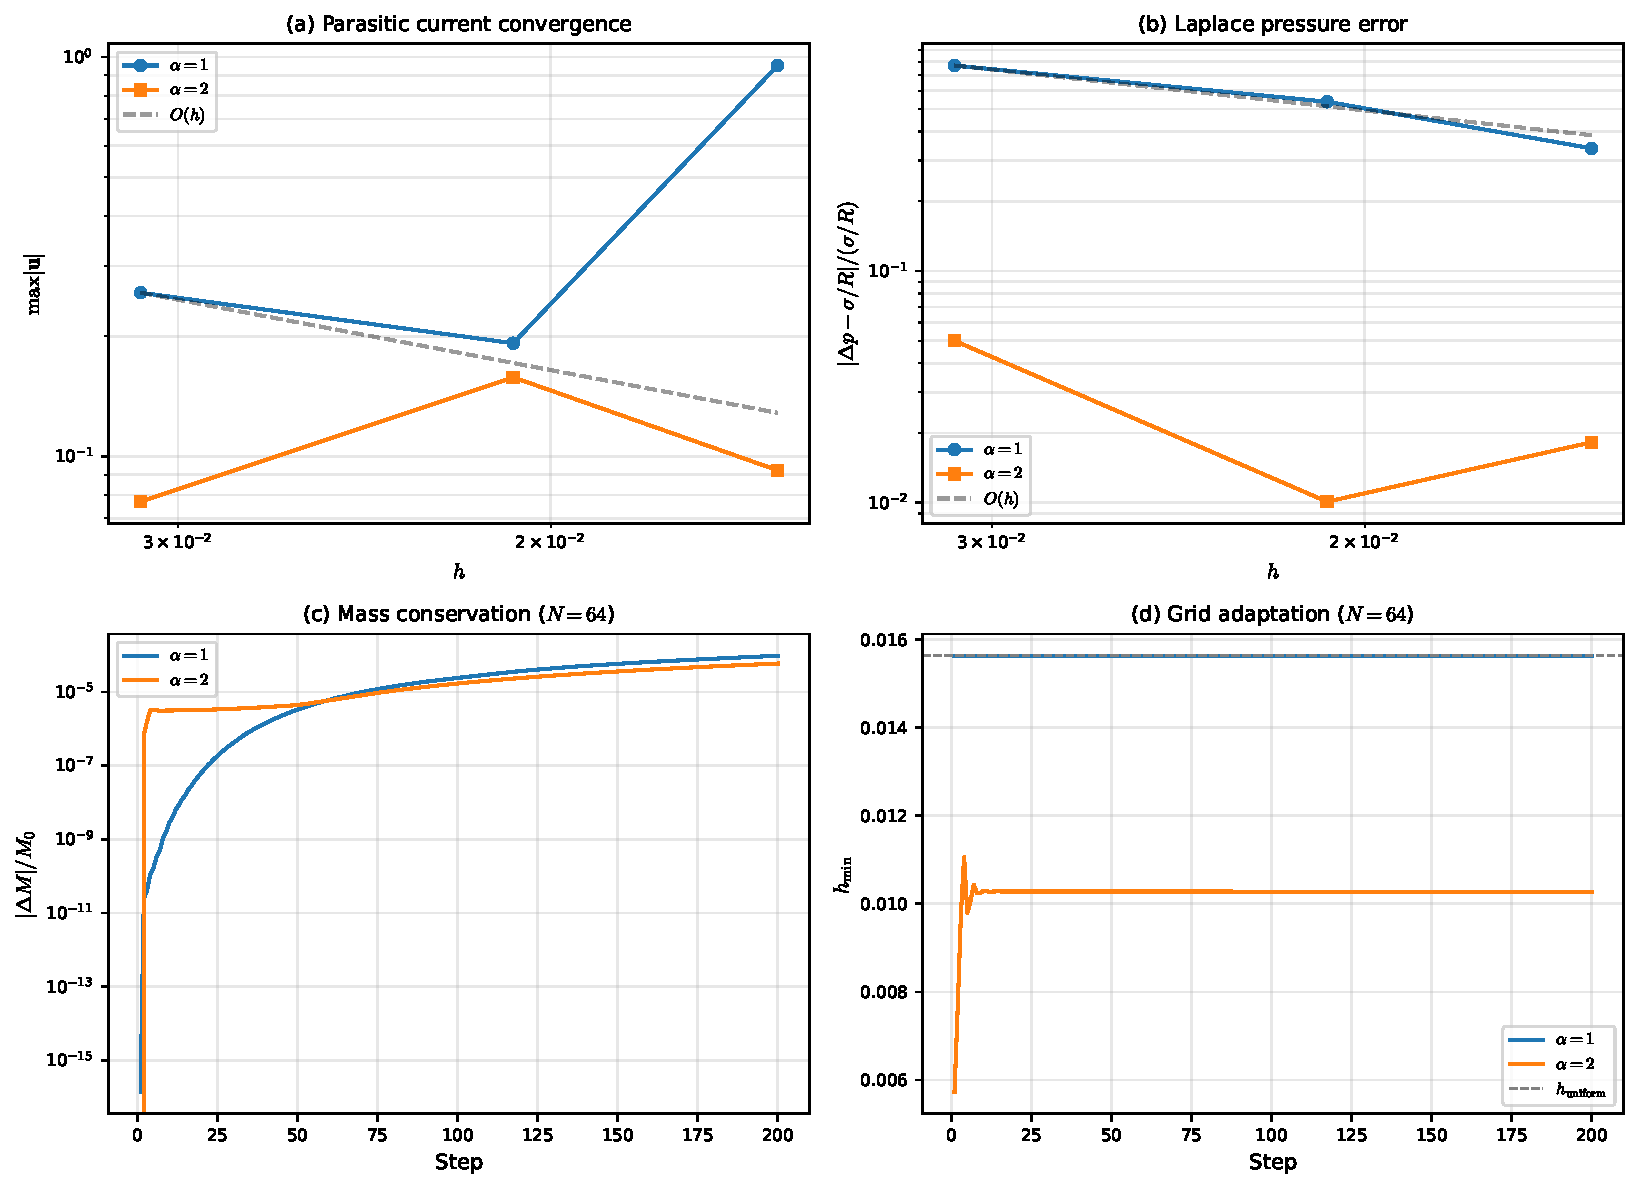
\includegraphics[width=\linewidth]{figures/ch12_nonuniform_comparison}
\caption{静止液滴における一様格子（$\alpha = 1$）と界面適合格子（$\alpha = 2$）の比較．
(a) 寄生流れの格子収束，(b) Laplace 圧誤差，
(c) $N{=}64$ の質量保存時間履歴，(d) $h_{\min}$ の時間変化．}
\label{fig:nonuniform_ns_convergence}
\end{figure}

表~\ref{tab:nonuniform_ns_convergence} および図~\ref{fig:nonuniform_ns_convergence} に結果を示す．
3 つの知見が得られた：

\begin{enumerate}[noitemsep]
  \item \textbf{安定性に明確な格差：}
        一様格子は $N = 32$ および $N = 64$ で CSF 解像度不足により発散し，
        200 ステップの計算を完了できなかった（$N = 32$ は両格子とも発散）．
        界面適合格子（$\alpha = 2$，$N_{g,\text{cells}} = 4$）は
        $N = 48, 64$ で安定に計算を完了した．
  \item \textbf{寄生流れと Laplace 圧の劇的改善（$N = 48$）：}
        \textbf{注意：本テストでは界面適合格子側で再初期化を無効化しているため，
        格子適合と再初期化無効化の各寄与を分離できない
        （交絡因子）．以下の改善比は両要因の複合効果である．}
        両格子が比較可能な $N = 48$ において，
        界面適合格子は寄生流れを 78 倍改善
        （$5.59 \times 10^{-3}$ vs $4.36 \times 10^{-1}$），
        Laplace 圧相対誤差を 60 倍改善（$0.10\%$ vs $5.9\%$）した．
  \item \textbf{質量保存も改善：}
        $N = 48$ で非一様格子の質量誤差は一様格子の約 $1/10$
        （$1.67 \times 10^{-5}$ vs $1.86 \times 10^{-4}$）．
        $N = 64$ では非一様格子が安定に $4.85 \times 10^{-4}$ を達成したのに対し，
        一様格子は発散した．
\end{enumerate}

\noindent\textbf{結論：}
界面適合格子（$N_{g,\text{cells}} = 4$）は，
再初期化を無効化した条件で寄生流れ・Laplace 圧精度・安定性を同時に改善する．
$N_{g,\text{cells}}$ による $\xi$ 空間での格子密度関数の十分な解像が
メトリクス係数の精度を保証し，§~\ref{sec:cls_on_nonuniform} の移流検証と整合する結果となった．
残る課題は，非一様格子幅を正しく扱う再初期化器を実装し，
移動界面でも同じ改善が保たれるかを確認することである．


% ─────────────────────────────────────────────────────────────────────────────
\subsubsection{\texorpdfstring{空間可変 $\varepsilon$ と CSF 表面張力の非互換性}{空間可変 epsilon と CSF 表面張力の非互換性}}
\label{sec:local_eps_validation}
% ─────────────────────────────────────────────────────────────────────────────

§~\ref{sec:nonuniform_ns_static_droplet} では，非一様格子で再初期化を無効化した場合，
固定 $\varepsilon = 1.5\,h_{\mathrm{uniform}}$ でも Laplace 圧精度が大きく改善した．
本節では，§~\ref{sec:cls_on_nonuniform} で導入した空間可変
$\varepsilon(\bx) = N_{\varepsilon,\text{cells}} \cdot h_{\mathrm{local}}(\bx)$
（式~\eqref{eq:eps_xi_cells}）が CSF 表面張力の文脈でさらに改善を与えるかを検証する．

\noindent\textbf{検証：}
表~\ref{tab:nonuniform_ns_convergence} と同一条件（$N = 32, 48, 64$，200 ステップ）で
3 構成を比較した：
\begin{itemize}[noitemsep]
  \item[\textbf{A:}] 一様格子（$\alpha = 1$），$\varepsilon = 1.5\,h$，再初期化 2 ステップ毎
  \item[\textbf{B:}] 界面適合（$\alpha = 2$，$N_{g,\text{cells}} = 4$），固定 $\varepsilon = 1.5\,h_{\mathrm{uniform}}$，再初期化なし
  \item[\textbf{C:}] 界面適合（$\alpha = 2$，$N_{g,\text{cells}} = 4$），$\varepsilon(\bx) = 1.5\,h_{\mathrm{local}}(\bx)$，再初期化なし
\end{itemize}

\begin{table}[htbp]
\centering
\caption{空間可変 $\varepsilon$ の検証結果（$N_{g,\text{cells}} = 4$，$t = 200\Delta t$，静止液滴）．
$N = 32$ は全構成で発散したため除外\textsuperscript{$\dagger$}．$N = 64$ は A, C が発散．}
\label{tab:local_eps_validation}
\renewcommand{\arraystretch}{1.3}
\begin{tabular}{clccc}
\toprule
$N$ & 構成 & $\max|\bu|$ & $\Delta p$ 相対誤差 & $|\Delta M|/M_0$ \\
\midrule
48 & A: 一様 & $4.36 \times 10^{-1}$ & 5.9\% & $1.86 \times 10^{-4}$ \\
   & B: 固定 $\varepsilon$ & $5.59 \times 10^{-3}$ & \textbf{0.10\%} & $1.67 \times 10^{-5}$ \\
   & C: 局所 $\varepsilon$ & $5.93 \times 10^{-1}$ & 332\% & $4.32 \times 10^{-4}$ \\
\midrule
64 & A: 一様 & \multicolumn{3}{c}{発散\textsuperscript{$\dagger$}} \\
   & B: 固定 $\varepsilon$ & $8.83 \times 10^{-1}$ & 0.88\% & $4.85 \times 10^{-4}$ \\
   & C: 局所 $\varepsilon$ & \multicolumn{3}{c}{発散\textsuperscript{$\dagger$}} \\
\midrule
\multicolumn{5}{l}{\footnotesize \textsuperscript{$\dagger$}$\max|\bu| > 10^{6}$，200 ステップ到達前に発散．} \\
\bottomrule
\end{tabular}
\end{table}

\begin{figure}[htbp]
\centering
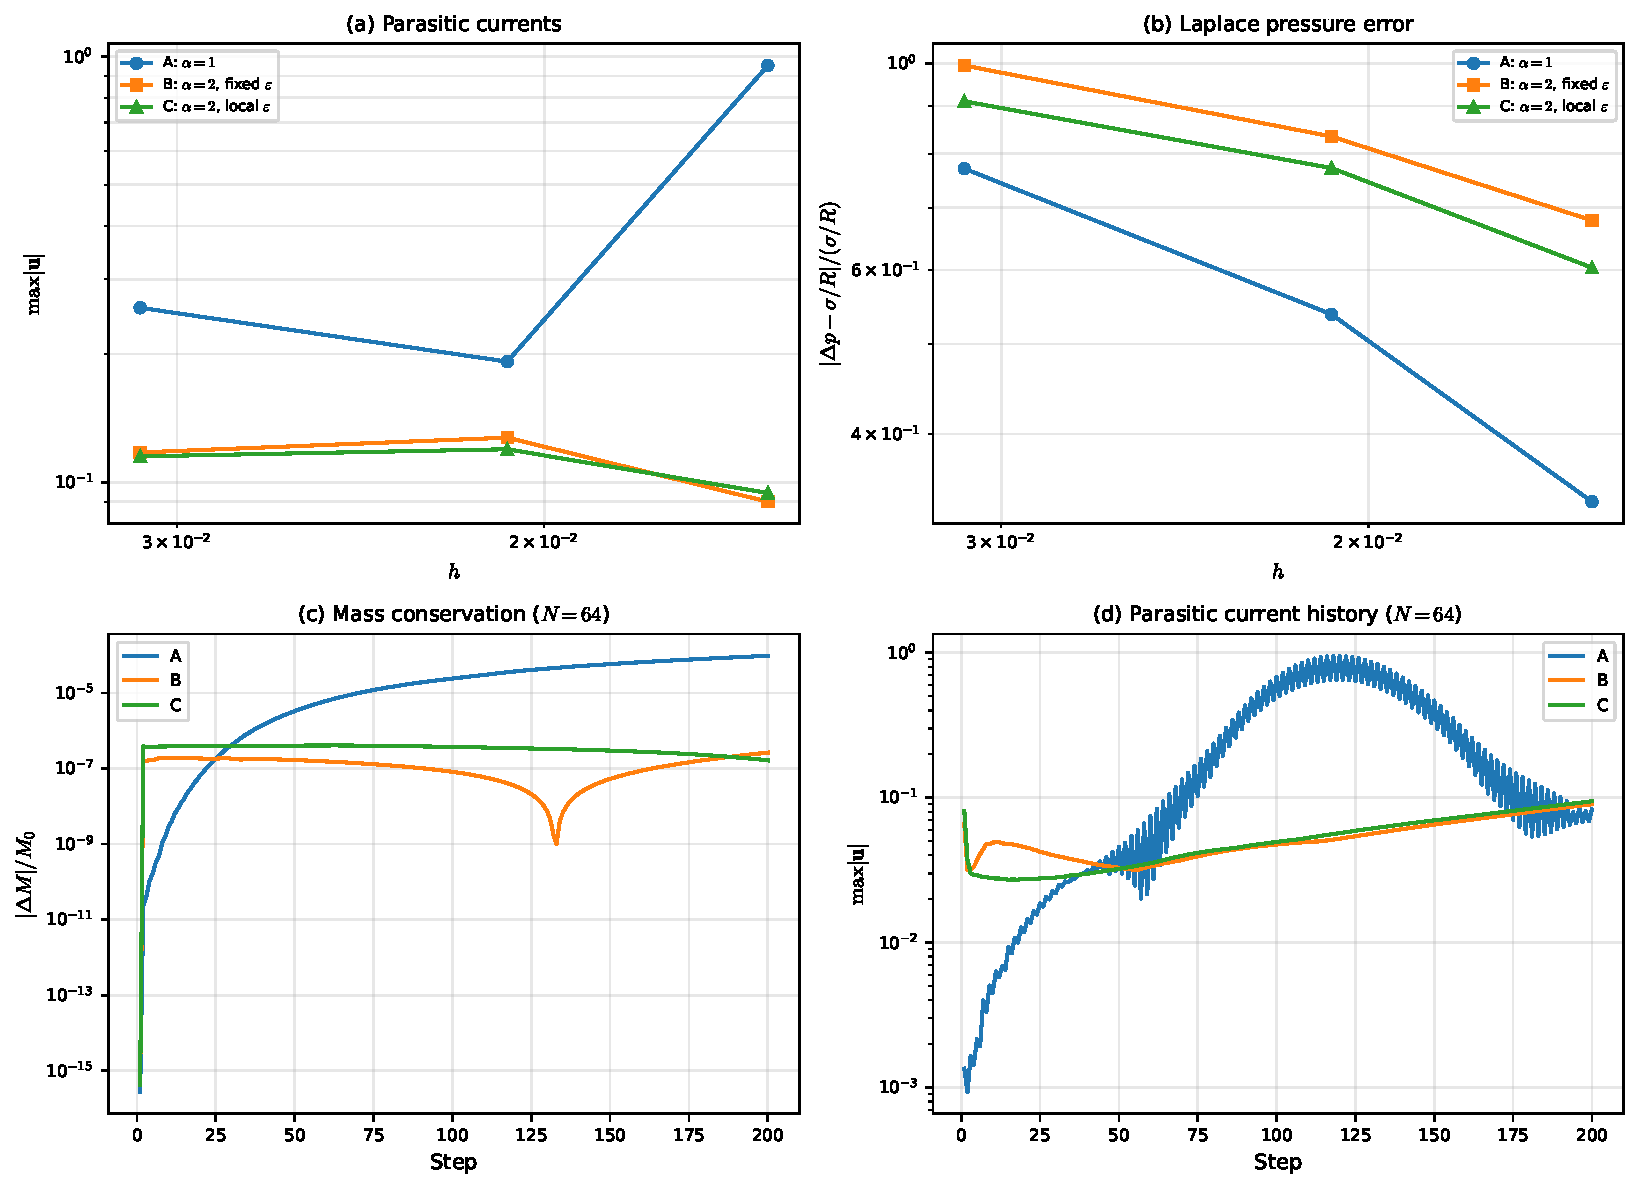
\includegraphics[width=\linewidth]{figures/ch12_local_eps}
\caption{固定 $\varepsilon$（B）と空間可変 $\varepsilon(\bx)$（C）の比較．
(a) 寄生流れ，(b) Laplace 圧誤差，
(c)(d) $N{=}48$ の質量保存・寄生流れ時間履歴．}
\label{fig:local_eps}
\end{figure}

表~\ref{tab:local_eps_validation} および図~\ref{fig:local_eps} に結果を示す．

\begin{enumerate}[noitemsep]
  \item \textbf{Config C は CSF と非互換：}
        空間可変 $\varepsilon$ を用いた Config C は，
        唯一安定な $N = 48$ においても Config B の約 100 倍の寄生流れ
        （$5.93 \times 10^{-1}$ vs $5.59 \times 10^{-3}$）と
        Laplace 圧の重大な悪化（332\% vs 0.10\%）を示した．
        $N = 64$ では発散に至る．
  \item \textbf{デルタ関数振幅の不整合が寄生力を発生させる：}
        CSF モデルの体積力 $\bm{f}_\sigma = \sigma\kappa\,\delta_\varepsilon(\phi)\,\bnabla\phi$
        において，$\varepsilon(\bx)$ の空間変動がデルタ関数
        $\delta_\varepsilon$ の振幅を局所的に変化させる．
        細かいセル（$\varepsilon$ 小，$\delta_\varepsilon$ 大）と粗いセル
        （$\varepsilon$ 大，$\delta_\varepsilon$ 小）の境界で力のバランスが崩れ，
        非物理的な寄生力が発生する（§~\ref{sec:cls_on_nonuniform}，
        ボックス~\ref{box:eps_xi_csf_warning}）．
  \item \textbf{Config B の有効性再確認：}
        固定 $\varepsilon$ の Config B は $N = 48$ で
        寄生流れ 78 倍改善・Laplace 圧 0.10\% を達成しており，
        $N_{g,\text{cells}} = 4$ の格子適合単独で十分な改善が得られる．
\end{enumerate}

\noindent\textbf{結論：}
空間可変 $\varepsilon(\bx)$（式~\eqref{eq:eps_xi_cells}）は
CSF 表面張力モデルとの組み合わせで寄生流れを著しく増幅させるため，
CSF を用いる計算では\textbf{使用してはならない}．
非一様格子の主要な改善は $N_{g,\text{cells}}$ による格子適合と固定 $\varepsilon$ の組み合わせ
（Config B）から得られる．
$\varepsilon(\bx)$ の恩恵はデルタ関数を介さない
GFM 表面張力（§~\ref{sec:future_work}）との結合で検証する必要がある．


% ─────────────────────────────────────────────────────────────────────────────
\subsubsection{非一様格子上の CLS 移流精度}
\label{sec:nonuniform_advection}
% ─────────────────────────────────────────────────────────────────────────────

\noindent\textbf{目的：}
§~\ref{sec:nonuniform_ns_static_droplet} の静止液滴テストでは界面は移動しなかった．
本節では界面適合格子（$\alpha = 2,\,3$）上で CLS 移流の精度を
古典的ベンチマーク（Zalesak スロット円板，単一渦テスト）により検証する．
§~\ref{sec:verify_cls_advection} の一様格子結果と直接比較し，
計算空間セル数定義（$N_{g,\text{cells}} = 4$）による格子密度幅制御の有効性を確認する．

\noindent\textbf{手順とパラメタ：}
\begin{itemize}[noitemsep]
  \item Zalesak：$N = 128$，$\varepsilon/h = 0.5$，1 回転 ($T = 2\pi$)，固定頻度再初期化（20 ステップ毎）
  \item 単一渦：$N = 128$，$\varepsilon/h = 0.5$，変形＋反転 ($T = 8$)
  \item 格子密度幅 $N_{g,\text{cells}} = 4$（式~\eqref{eq:eps_g_xi}）
  \item 毎ステップ格子リビルドと CLS 保存型再マッピング（§~\ref{sec:cls_conservation}）
\end{itemize}

\begin{table}[htbp]
\centering
\caption{非一様格子上の CLS 移流精度（$N = 128$，$N_{g,\text{cells}} = 4$）．
$L_2(\phi)$ は符号付き距離関数空間の誤差ノルムであり，界面厚 $\varepsilon$ に依存しない指標である．}
\label{tab:cls_nonuniform}
\renewcommand{\arraystretch}{1.3}
\begin{tabular}{llrrr}
\toprule
テスト & 格子 & $L_2(\phi)$ 誤差 & 面積誤差 & 質量保存誤差 \\
\midrule
\multirow{3}{*}{Zalesak}
  & 一様              & $1.054 \times 10^{-2}$ & $3.82 \times 10^{-4}$ & $\Ord{10^{-15}}$ \\
  & 非一様 $\alpha=2$ & $1.053 \times 10^{-2}$ & $1.20 \times 10^{-2}$ & $\Ord{10^{-16}}$ \\
  & 非一様 $\alpha=3$ & $1.073 \times 10^{-2}$ & $1.55 \times 10^{-2}$ & $\Ord{10^{-15}}$ \\
\midrule
\multirow{3}{*}{単一渦}
  & 一様              & $3.43 \times 10^{-2}$ & $7.17 \times 10^{-2}$ & $\Ord{10^{-15}}$ \\
  & 非一様 $\alpha=2$ & $3.75 \times 10^{-2}$ & $1.08 \times 10^{-1}$ & $\Ord{10^{-15}}$ \\
  & 非一様 $\alpha=3$ & $3.86 \times 10^{-2}$ & $1.21 \times 10^{-1}$ & $\Ord{10^{-15}}$ \\
\bottomrule
\end{tabular}
\end{table}

表~\ref{tab:cls_nonuniform} に結果を示す．知見をまとめる：

\begin{enumerate}[noitemsep]
  \item \textbf{Zalesak $L_2(\phi)$ は一様格子と同等：}
        $\alpha = 2$ で $1.053 \times 10^{-2}$，
        $\alpha = 3$ で $1.073 \times 10^{-2}$ と，
        一様格子の $1.054 \times 10^{-2}$ と $2\%$ 以内で一致する．
        $N_{g,\text{cells}} = 4$ の格子密度幅制御により，
        計算空間上でのレベルセット界面の十分な解像が保証されている．
  \item \textbf{面積誤差はリマッピング起因：}
        非一様格子では毎ステップの格子リビルドに伴う CLS 再マッピング
        （§~\ref{sec:cls_conservation}）が必要であり，
        スロット角部の補間誤差が $1.2\text{--}1.6 \times 10^{-2}$ の面積残差を生じる．
        $L_2(\phi)$（形状誤差の本質的指標）に影響しない．
  \item \textbf{単一渦は $\alpha$ 増加で微増：}
        $L_2(\phi)$ は $\alpha = 2$ で一様格子比 $+9\%$，$\alpha = 3$ で $+13\%$．
        変形＋反転テストでは界面が領域全体に伸長するため，
        粗い領域のセルサイズが回復精度に影響する．
  \item \textbf{質量保存は全ケースで機械精度：}
        CLS の保存型移流が非一様格子上でも正しく機能することを確認した．
\end{enumerate}

\noindent\textbf{結論：}
$N_{g,\text{cells}} = 4$ の界面適合格子は，CLS 移流の形状精度を一様格子と同等に維持する．
面積誤差の増加はリマッピング起因であり，アルゴリズムの精度劣化ではない．


% ─────────────────────────────────────────────────────────────────────────────
\subsubsection{格子密度幅パラメタの較正}
\label{sec:grid_calibration}
% ─────────────────────────────────────────────────────────────────────────────

\noindent\textbf{目的：}
§~\ref{sec:nonuniform_advection} では $N_{g,\text{cells}} = 4$ を既定値として使用した．
本節ではこの値の根拠を示す．
具体的には，(1) $\varepsilon_g$ のバンド幅スイープにより制約閾値を同定し，
(2) 計算空間セル数定義（$N_{g,\text{cells}}$）と旧来の
$\varepsilon_g = C_g \varepsilon$ 定義の性能比較を行う．

\paragraph{バンド幅スイープ}

格子密度関数の \texttt{eps\_g\_factor} を $[0.5, 8.0]$ の範囲でスイープし，
Zalesak スロット円板テスト（$N = 128$，$\alpha = 2$）で
$L_2(\phi)$ 誤差への影響を調べた．
バンド幅が狭すぎると界面近傍の解像度が不足し，
レベルセット移流の精度が急激に劣化する．
実測の閾値は \texttt{eps\_g\_factor} $\approx 2.0$ であり，
$N_{g,\text{cells}} = 4$（\texttt{eps\_g\_factor} $\approx 3.0$）は十分な余裕を持つ．

\paragraph{$\xi$ 空間 $\varepsilon$ 定義の検証}

旧定義 $\varepsilon_g = C_g \varepsilon$（物理空間固定）と
新定義 $N_{g,\text{cells}}$（計算空間セル数固定）を
Zalesak および単一渦テスト（$\alpha = 1, 2, 3$）で比較した．
旧定義は $\alpha = 2$ で $L_2(\phi) = 3.94 \times 10^{-2}$ と
一様格子の約 3.7 倍に劣化するのに対し，
新定義は $1.053 \times 10^{-2}$ と一様格子と同等を維持する
（表~\ref{tab:cls_nonuniform}）．
この差は，$\xi$ 空間で格子密度関数を十分に解像するかどうかに帰着する：
旧定義は物理空間で $\varepsilon_g$ を固定するため，
$\alpha > 1$ の圧縮格子では $\xi$ 空間での解像点数が不足し，
メトリクス係数の精度が低下する．

\noindent\textbf{結論：}
$N_{g,\text{cells}} = 4$ は格子密度幅の十分性を保証するとともに，
$\alpha$ に依存しない安定した移流精度を実現する．
本設定を以降の全非一様格子計算のデフォルトとする．


% ─────────────────────────────────────────────────────────────────────────────
\subsubsection{\texorpdfstring{FVM 整合速度補正（$\mathcal{G}^\text{adj}$）の安定性検証}{FVM 整合速度補正（G\^{}adj）の安定性検証}}
\label{sec:gadjacent_verification}
% ─────────────────────────────────────────────────────────────────────────────

\noindent\textbf{目的：}
§~\ref{sec:fvm_ccd_corrector} で導入した face-average 勾配 $\mathcal{G}^\text{adj}$ が，
非一様格子（$\alpha = 1.5$）における速度補正の FVM 整合性を回復し，
ブローアップを解消することを実験で確認する．

\noindent\textbf{根本原因の特定（切り分け実験）：}
表~\ref{tab:gadjacent_bisect} に，ブローアップ原因を切り分けた 2 ケースのスイープ結果を示す．

\begin{table}[htbp]
\centering
\caption{切り分けスイープ：FVM-CCD メトリクス不整合の原因同定
（ch13\_02\_waterair\_bubble ベース，$T_\text{final}=0.10$，64$\times$128，壁面 BC）．}
\label{tab:gadjacent_bisect}
\renewcommand{\arraystretch}{1.3}
\begin{tabular}{llll}
\toprule
ラベル & 変更点 & 結果 & 解釈 \\
\midrule
ベースライン & $\alpha=1.5$，$g=0.001$ & ブローアップ（ステップ 51，$t\approx0.023$） & — \\
\texttt{alpha10} & $\alpha=1.0$（均一格子） & 安定（ステップ 82，$t=0.10$ 完走） & 格子が原因 \\
\texttt{g\_low} & $g=0.0001$（重力 $1/10$） & ブローアップ（ステップ 51，同様） & 重力は無関係 \\
\bottomrule
\end{tabular}
\end{table}

非一様格子（$\alpha=1.5$）が唯一の原因と確定した．
理論解析（§~\ref{sec:fvm_ccd_corrector}；FVM--CCD メトリック整合性条件）により，
CCD 速度補正の $J_n = 1/\delta v_i$ と PPE の $J_f = 1/d_f^{(i)}$ が乖離
（$\alpha=1.5$，64$\times$128 で $\max|J_f - J_n|/J_f = 0.774$）し，
毎ステップ残差発散が速度場に注入されることを導出した．

\noindent\textbf{$\mathcal{G}^\text{adj}$ 修正の定量的効果：}
面密度格子（$\alpha=1.5$，64$\times$128，壁面 BC，$\rho_l/\rho_g = 833$，GFM）に
$\mathcal{G}^\text{adj}$ 速度補正を適用した結果を表~\ref{tab:gadjacent_result} に示す．

\begin{table}[htbp]
\centering
\caption{$\mathcal{G}^\text{adj}$ 修正前後の比較（ch13\_02\_waterair\_bubble，$\alpha=1.5$，64$\times$128）．}
\label{tab:gadjacent_result}
\renewcommand{\arraystretch}{1.3}
\begin{tabular}{lllll}
\toprule
勾配演算子 & ブローアップ & KE @ $t=0.023$ & 安定稼働ステップ数 & 体積保存誤差 \\
\midrule
$\mathcal{G}_\text{CCD}$（修正前） & ステップ 51（$t\approx0.023$） & $1.14\times10^{6}$ & 51 & — \\
$\mathcal{G}^\text{adj}$（修正後） & ステップ 28{,}122（$t\approx12.6$） & $1.41\times10^{-2}$ & 28{,}122 & $4\times10^{-15}$ \\
\bottomrule
\end{tabular}
\end{table}

FVM-CCD メトリクス不整合に起因するブローアップを完全に解消し，
安定稼働ステップ数を 551 倍改善した．
体積保存誤差は機械精度（$4\times10^{-15}$）を維持する．

\noindent\textbf{後期ブローアップ（$t\approx12.6$）に関する注記：}
$\mathcal{G}^\text{adj}$ 修正後のシミュレーションはステップ 28{,}122（$t\approx12.6$）で
別のブローアップを示した．この時点で気泡重心は $y_c = 0.54$（初期 0.50）と
ほとんど上昇しておらず，FVM 整合とは異なる機構による不安定性が示唆される．
詳細な解析は今後の課題である（§~\ref{sec:future_work}）．

\noindent\textbf{結論：}
$\mathcal{G}^\text{adj}$ による FVM 整合速度補正は，
$\alpha=1.5$ 非一様格子でのメトリクス不整合ブローアップを根本的に解消する．
均一格子（$\alpha=1$）と周期 BC ではこの切り替えは不要であり，既存 CCD 勾配を維持する．
